\subsection{SP5: transporte cooperativo de carga extendida}
\label{sec:resultados-sp5}

\subsubsection{Frontera SP4--SP5 y planta}

SP5 v2 comienza después del acoplamiento: los robots ocupan contactos fijos en el marco de la carga y no se vuelve a evaluar el reclutamiento. La postura $q=(x,y,\theta)$ sigue
\[
 M\ddot q+D\dot q=w_{\rm EXEC}+d.
\]
El controlador produce $w_{\rm RAW}$, el filtro de barrera produce $w_{\rm SAFE}$ y el reparto de fuerzas acotadas produce $w_{\rm EXEC}=G(q)u$. Solo EXEC mueve la planta. No existe proyección de posiciones posterior a la integración.

Para el regulador Hamiltoniano se usa $V=\tfrac12(q-q_d)^\top K(q-q_d)$, $p=M\dot q$ y
\[
 \mathcal H(q,p)=\tfrac12p^\top M^{-1}p+V(q).
\]
La disipación nominal no constituye una propiedad automática de EXEC: el filtro y la saturación modifican el \emph{wrench}. Por ello, la seguridad se decide mediante despeje observado y las colisiones se conservan.

\subsubsection{Protocolo congelado}

El piloto corrigió la envolvente de seguridad para cubrir el compuesto carga--robots y el espaciado de contactos antes del freeze. La campaña confirmatoria fijó seis escenarios, $N\in\{4,8,12\}$, seis semillas nuevas y ocho métodos. Los 108 mundos compartidos generaron 864 ejecuciones CPU. El manifiesto congelado precede al evento de apertura; todos los timeouts y colisiones permanecen en el denominador.

\begin{figure}[tbp]
\centering
\begin{minipage}[t]{0.49\textwidth}
\centering
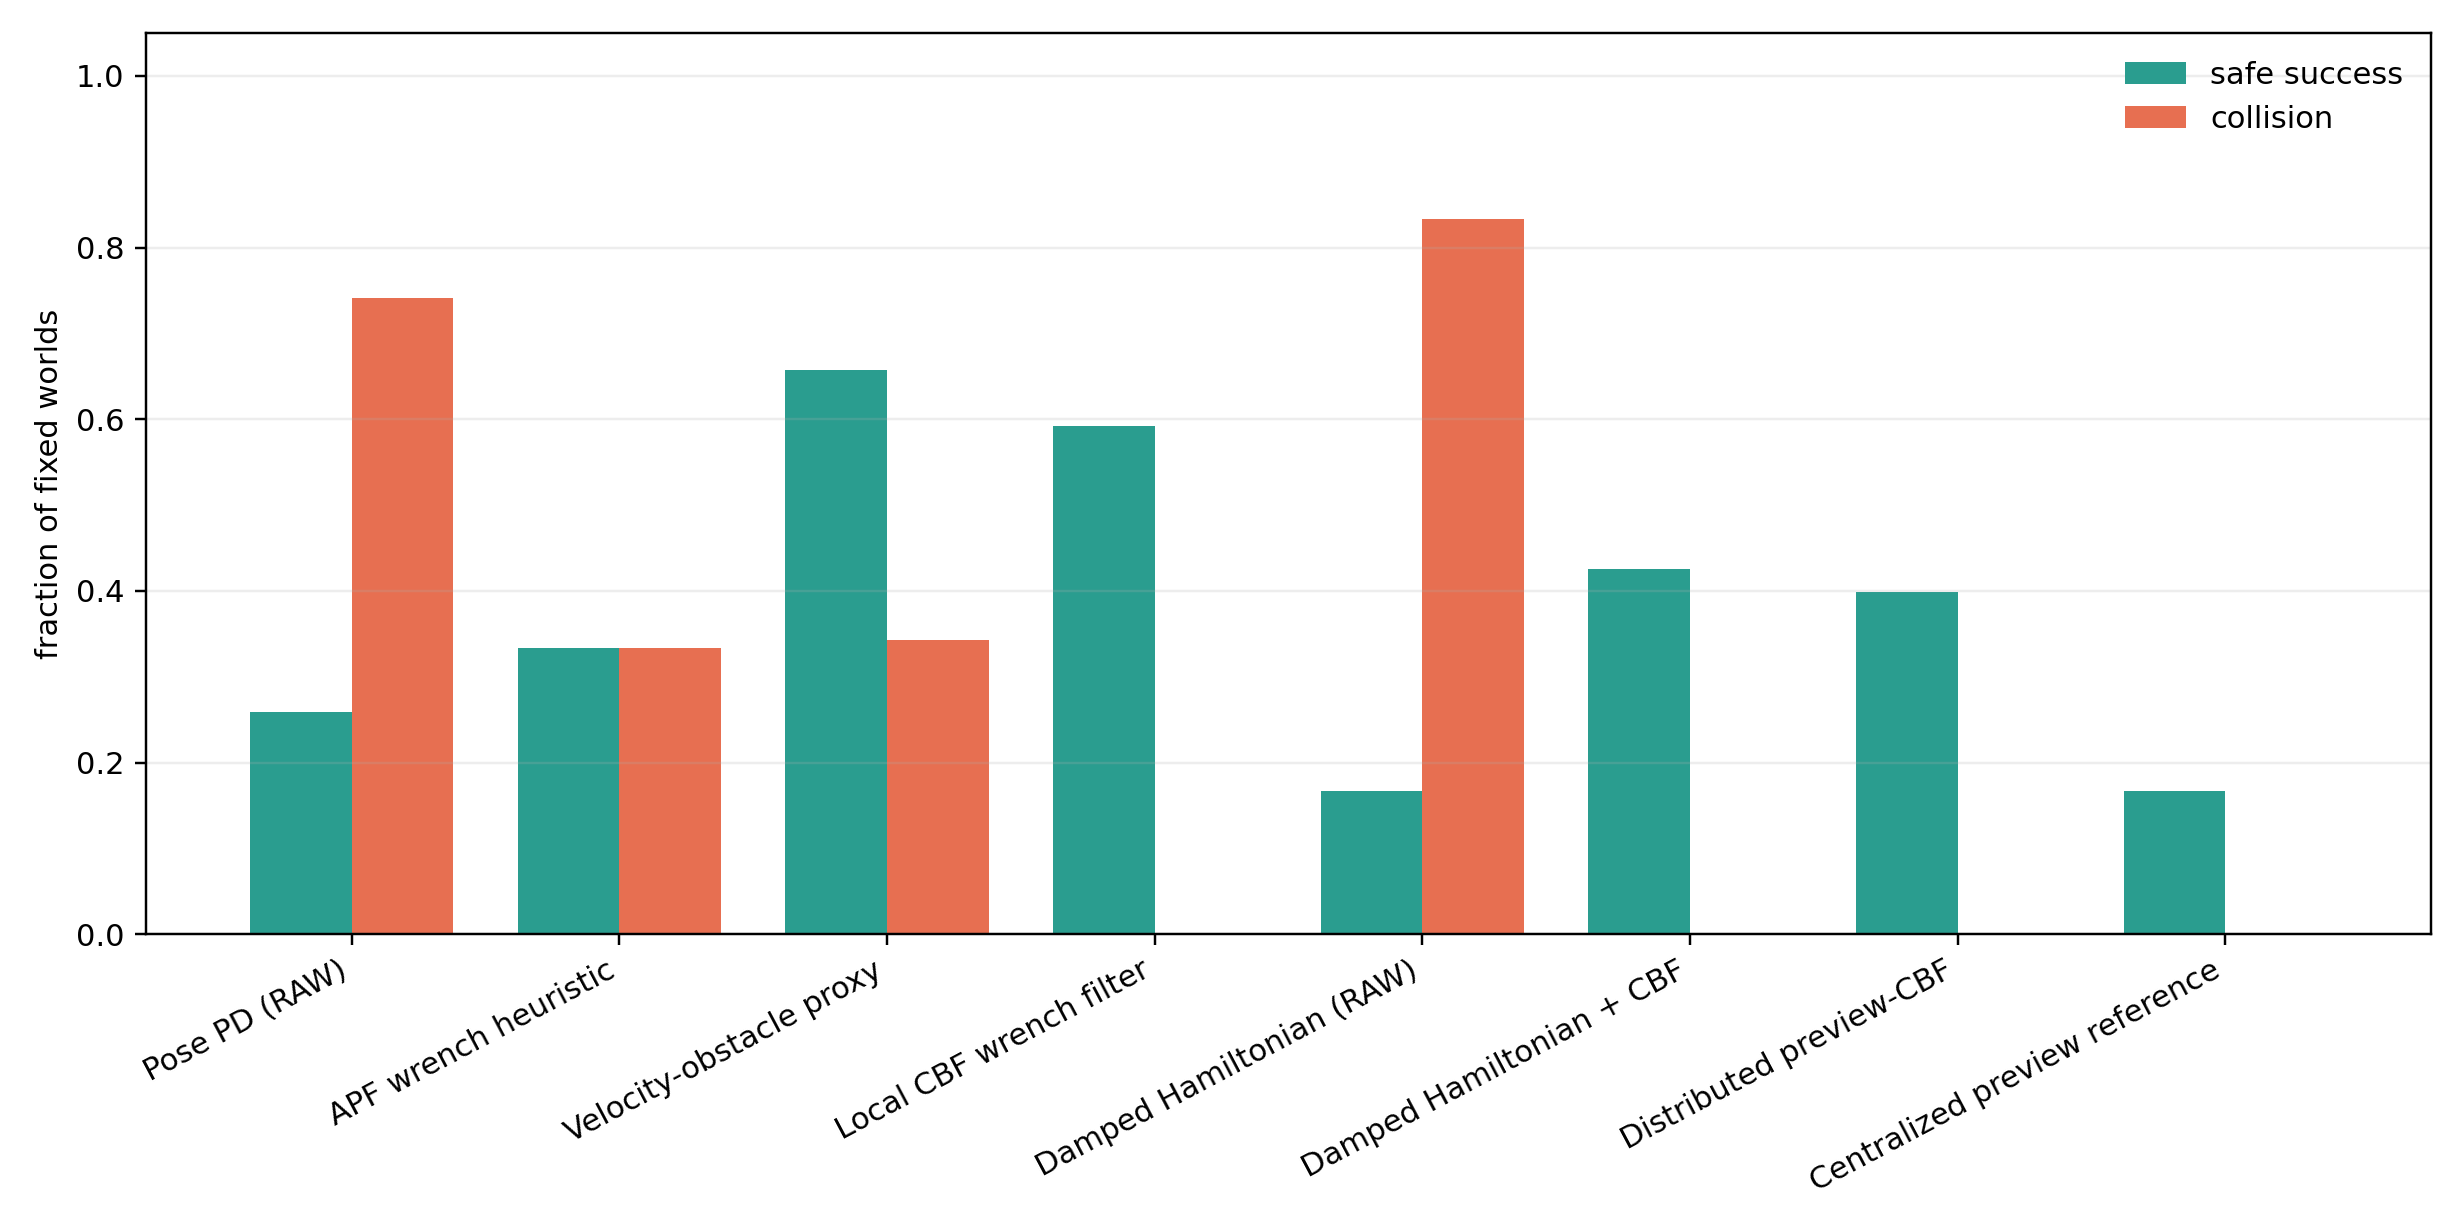
\includegraphics[width=\linewidth]{figures/fig-sp5-primary.png}
\end{minipage}\hfill
\begin{minipage}[t]{0.49\textwidth}
\centering
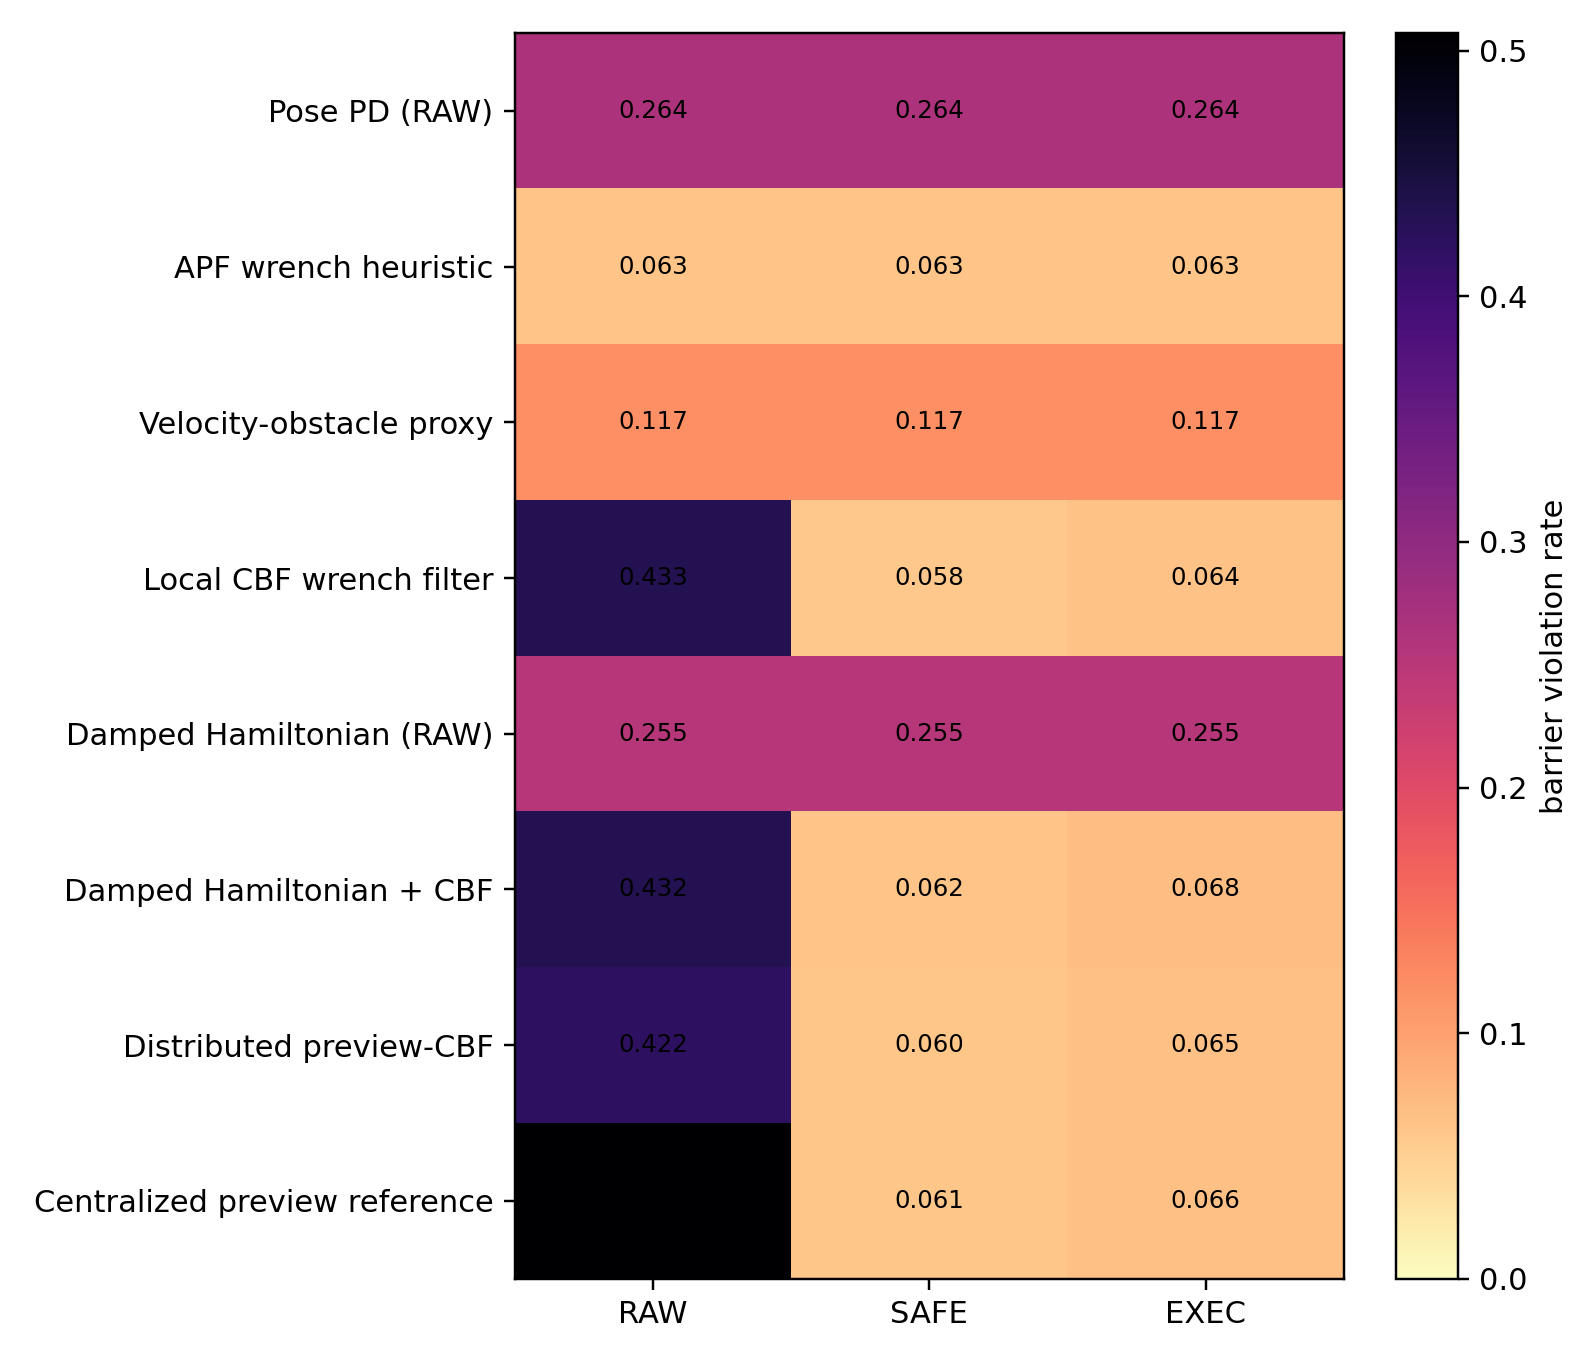
\includegraphics[width=\linewidth]{figures/fig-sp5-raw-safe-exec.png}
\end{minipage}
\caption[SP5 v2: rendimiento y etapas]{Rendimiento ejecutado y separación RAW--SAFE--EXEC.}
\viuownsource
\label{fig:sp5-v2-expanded}
\end{figure}

\subsubsection{Resultados y límites}

CBF local alcanzó $0{,}593$ de éxito seguro y cero colisiones. El proxy VO obtuvo $0{,}657$, con $0{,}343$ de colisiones. Hamiltoniano RAW obtuvo $0{,}167$ de éxito y $0{,}833$ de colisión; Hamiltoniano+CBF obtuvo $0{,}426$ y cero colisiones. Holm respaldó la reducción de colisión y la mejora de éxito frente a RAW, además de la reducción de colisiones del preview distribuido frente a VO. No respald\'o que la referencia centralizada superara al CBF local ni la direcci\'on del contraste CBF--APF. En este \`ultimo, $p_{\rm Holm}=0{,}0038$ no revierte la decisi\'on: el efecto medio tuvo el signo contrario ($+0{,}0012$) y su IC95\% $[-0{,}0305,0{,}0390]$ incluy\'o cero.

El residual máximo de la identidad mecánica discreta fue $1{,}14\times10^{-13}$. Este resultado verifica coherencia numérica del modelo, no contacto realista. No se modelan cono de fricción, dinámica de rueda, deformación, carga tridimensional ni seguridad funcional. El paquete histórico de 20.040 filas se conserva como no canónico porque reparaba geométricamente las poses tras integrar.
